\documentclass[tikz, border=10pt]{standalone}
\usepackage{tikz}
\usepackage{amsmath}
\usepackage{amssymb}
\usetikzlibrary{calc}

% Conditional risks of the two actions in binary classification as functions
% of eta_1 = P(Y = 1 | x), with C_00 = C_11 = 0:
%   R(0 | x) = C_10 eta_1(x),   R(1 | x) = C_01 (1 - eta_1(x)).
% Panel (a): C_01 = C_10 = 1, crossing at 0.5. Panel (b): C_10 = 10 and
% C_01 = 1, crossing at 1/11. The risk axis is cut at 1.15, so in (b) the
% line 10 eta_1 leaves the picture at eta_1 = 0.115. The thresholds are
% written as numbers because p* is defined on a later frame.
\begin{document}
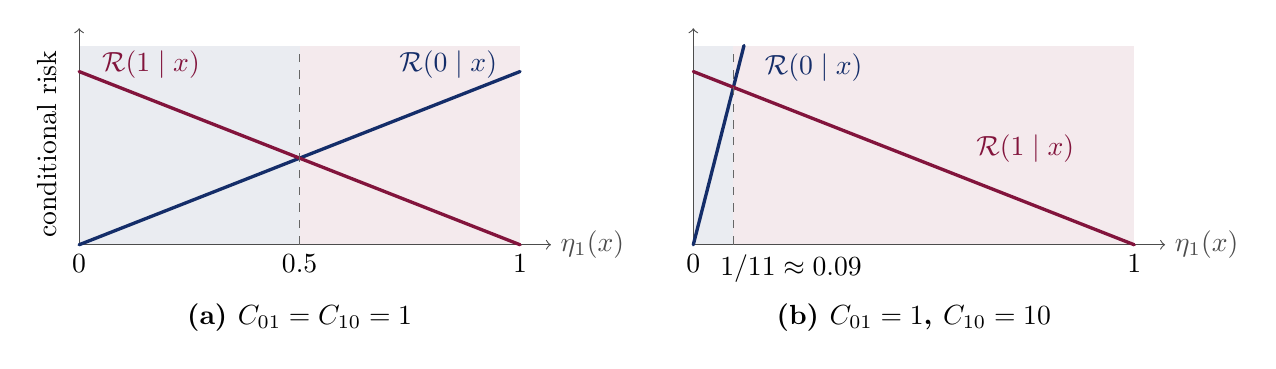
\begin{tikzpicture}[font=\sffamily, x=5.6cm, y=2.2cm,
    risk/.style={very thick, line cap=round},
    axis/.style={->, black!70},
    lbl/.style={font=\normalsize}]
  \definecolor{actzero}{HTML}{142D69}
  \definecolor{actone}{HTML}{82143C}

  % ---- (a) both errors cost the same ----
  \begin{scope}
    \fill[actzero!9] (0, 0) rectangle (0.5, 1.15);
    \fill[actone!9] (0.5, 0) rectangle (1, 1.15);
    \draw[axis] (0, 0) -- (1.07, 0) node[right, lbl] {$\eta_1(x)$};
    \draw[axis] (0, 0) -- (0, 1.25);
    \node[lbl, rotate=90, anchor=south] at (-0.03, 0.58) {conditional risk};
    \draw[risk, actzero] (0, 0) -- (1, 1);
    \draw[risk, actone] (0, 1) -- (1, 0);
    \draw[dashed, black!60] (0.5, 0) -- (0.5, 1.15);
    % Line labels in the top band.
    \node[lbl, actone, anchor=west] at (0.03, 1.04) {$\mathcal{R}(1 \mid x)$};
    \node[lbl, actzero, anchor=east] at (0.97, 1.04) {$\mathcal{R}(0 \mid x)$};
    \node[below, lbl] at (0, 0) {$0$};
    \node[below, lbl] at (1, 0) {$1$};
    \node[below, lbl] at (0.5, 0) {$0.5$};
    \node[lbl, font=\normalsize\bfseries] at (0.5, -0.42)
      {(a) $C_{01} = C_{10} = 1$};
  \end{scope}

  % ---- (b) a false negative costs ten times more ----
  \begin{scope}[xshift=7.8cm]
    \fill[actzero!9] (0, 0) rectangle (0.0909, 1.15);
    \fill[actone!9] (0.0909, 0) rectangle (1, 1.15);
    \draw[axis] (0, 0) -- (1.07, 0) node[right, lbl] {$\eta_1(x)$};
    \draw[axis] (0, 0) -- (0, 1.25);
    \draw[risk, actzero] (0, 0) -- (0.115, 1.15);
    \draw[risk, actone] (0, 1) -- (1, 0);
    \draw[dashed, black!60] (0.0909, 0) -- (0.0909, 1.15);
    \node[lbl, actzero, anchor=west] at (0.14, 1.02) {$\mathcal{R}(0 \mid x)$};
    \node[lbl, actone, anchor=south west] at (0.62, 0.42)
      {$\mathcal{R}(1 \mid x)$};
    \node[below, lbl] at (0, 0) {$0$};
    \node[below, lbl] at (1, 0) {$1$};
    \node[below, lbl, anchor=north west, inner xsep=0pt] at (0.06, 0)
      {$1/11 \approx 0.09$};
    \node[lbl, font=\normalsize\bfseries] at (0.5, -0.42)
      {(b) $C_{01} = 1$, $C_{10} = 10$};
  \end{scope}
\end{tikzpicture}
\end{document}
